\section{Requirements}
\label{sec:eval_requirements} 

Please note that the exact requirement calculation methods are quite complex and will be added at a later point. \\

\subsection{Detection}
\label{sec:eval_req_detection} 

\subsubsection{Configuration}

\begin{figure}[H]
    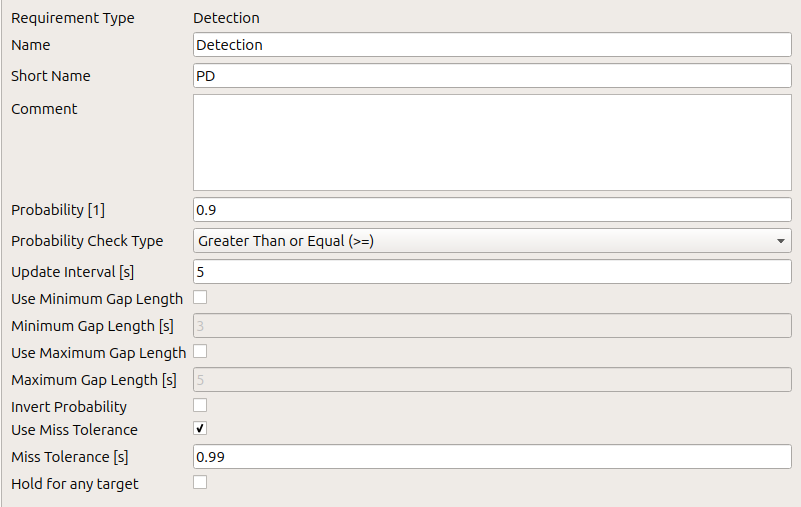
\includegraphics[width=14cm,frame]{figures/eval_req_detection.png}
  \caption{Evaluation Detection requirement}
\end{figure}

The 'Detection' requirement can be used to check whether targets are detected at all. For each target existing in the reference data (within the current sector) a target must be detected within e.g. each test update interval or other given interval. Missed update intervals are either called misses or gaps, which are used to calculate a probability of detection, which has to fulfill a given threshold. \\

\begin{itemize}  
\item Probability [1]: Probability of detection
\item Probability Check Type: $\geq$
\item Update Interval [s]: Update interval of the test data
\item Use Minimum Gap Length: Checkbox if minimum gap length should be used
\item Minimum Gap Length [s]: Minimum gap length to be considered
\item Use Maximum Gap Length: Checkbox if maximum gap length should be used
\item Maximum Gap Length [s]: Maximum gap length to be considered
\item Use Miss Tolerance: Checkbox if miss tolerance should be used
\item Miss Tolerance [s]: Acceptable time delta for miss detection
\end{itemize}
\ \\

\subsubsection{Calculation}

As a summary, the reference is used to calculate the number of expected update intervals inside the sector layer (\#EUI). Then, for the test data, if the reference exists at the time, time differences between target reports are checked and the number of misses/gaps are calculated as number of missed update intervals (\#MUI). \\

Gaps are, if a minimum or maximum gap length is used, only counted if the detected gap fulfills the thresholds. \\

The ratio of \#MUI and \#EUI gives the probability of missed update interval, the counter-probability gives the Probability of Detection (PD). The PD must greator or equal than the defined 'Probability' for the requirement to pass.

\subsubsection{Result Values}

\paragraph{Sector}

\begin{center}
 \begin{table}[H]
  \begin{tabularx}{\textwidth}{ | l | X |  l | }
    \hline
    \textbf{Name} & \textbf{Description} & \textbf{Example} \\ \hline
    Sector Layer & Name of the sector layer & fir\_cut\_sim \\ \hline
    Reqirement Group & Name of the requirement group & Mandatory  \\ \hline
    Reqirement & Name of the requirement & Detection  \\ \hline
    Num Results & Total number of results & 728  \\ \hline
    Num Usable Results & Number of usable results & 417  \\ \hline
    Num Unusable Results & Number of unusable results & 311  \\ \hline
    \#Updates/\#EUIs [1] & Total number update intervals & 7960  \\ \hline
    \#MUIs [1] & Number of missed update intervals & 2221  \\ \hline
    PD [\%] & Probability of Detection & 72.10  \\ \hline
    Condition &  & >= 90.00  \\ \hline
    Condition Fulfilled &  & Failed  \\ \hline
\end{tabularx}
\end{table}
\end{center}

Also, a table is given for all single targets, sorted by PD.

\paragraph{Single Target}

\begin{center}
 \begin{table}[H]
  \begin{tabularx}{\textwidth}{ | l | X |  l | }
    \hline
    \textbf{Name} & \textbf{Description} & \textbf{Example} \\ \hline
    Use & To be used in results & true \\ \hline
    \#EUIs [1] & Expected Update Intervals & 6 \\ \hline
    \#MUIs [1] & Missed Update Intervals & 5 \\ \hline
    PD [\%] & Probability of Detection & 16.67 \\ \hline
    Reference Period 0 & Time inside sector & [15:47:22.680,15:47:45.828] \\ \hline
    Reference Period 1 & Time inside sector & [15:47:53.844,15:47:57.844] \\ \hline
    Condition &  & >= 90.00 \\ \hline
    Condition Fulfilled &  & Failed \\ \hline
\end{tabularx}
\end{table}
\end{center}

%-------

\subsection{Dubious Targets}
\label{sec:eval_req_dubious_targets} 

\subsubsection{Configuration}

\begin{figure}[H]
    \includegraphics[width=14cm,frame]{figures/eval_req_dubious_targets.png}
   \caption{Evaluation Dubious Targets}
\end{figure}

The 'Dubious Targets' requirement can be used to check for dubious for dubious movement from data-source. This requirement checks based on test data only, so the reference data is of no importance. \\

For each track number (existing in an UTN) a number of checks are performed, and a probability of dubious target report is calculated. Which checks are used can be defined as follows, but are focused on short tracks or physically dubious movement. \\

\begin{itemize}  
\item Probability [1]: Probability of dubious target
\item Probability Check Type: $\geq$
\item Minimum Comparison Time [s]: Skip movement checks if time between updates is smaller than the defined time
\item Maximum Comparison Time [s]: Skip movement checks if time between updates is larger than the defined time
\item Mark Primary-Only: Checkbox if all primary-only tracks should be counted as dubious
\item Use Minimum Updates: Checkbox if tracks with less than the defined number of updates should be counted as dubious
\item Minimum Updates [1]: Minimum number of updates
\item Use Minimum Duration: Checkbox if tracks with a duration less than the defined time should be counted as dubious
\item Minimum Duration [s]: Minimum duration
\item Use Maximum Groundspeed: Checkbox if maximum groundspeed should be used
\item Maximum Groundspeed [kts]: Maximum groundspeed to be considered
\item Use Maximum Acceleration: Checkbox if maximum acceleration should be used
\item Maximum Acceleration [$m/s^{2}$]: Maximum acceleration to be considered
\item Use Maximum Turnrate: Checkbox if maximum turnrate should be used
\item Turnrate Groundspeed [deg/s]: Maximum groundspeed to be considered
\item Use Maximum ROCD: Checkbox if turnrate rate of climb/descent should be used
\item Maximum ROCD [ft/s]: Maximum  rate of climb/descent to be considered
\item Dubious Probability [1]: Probability of dubious target report to classify a track as dubious
\end{itemize}
\ \\

\subsubsection{Calculation}

As a summary, the test data is used to calculate the number of dubious targets in relation to the total number of targets, which gives the probability of dubios target (PDT). If this probability is larger than the required one, the requirement is failed. \\

A track is be ignored (from dubious detection) if the last-updating sensor parameter is active, and the track was updated by at any point by any other sensor. \\

The total track updates are marked as dubious if any of the following cases hold:
\begin{itemize}  
\item 'Mark Primary-Only' is used, and the track is always primary-only (no secondary attributes)
\item 'Minimum Updates' are used, and the number of track updates is smaller than the required threshold
\item 'Minimum Duration' is used, and the duration of the track is smaller than the required threshold
\end{itemize}
\ \\

For the movement checks, for each track update the movement is checked. If the Minimum/Maximum Comparison Time check fails, the respective track update is skipped (not checked). \\ 

The following checks can be performed:
\begin{itemize}  
\item 'Maximum Groundspeed': The track update's groundspeed (as output from the data source, as well as calculated from position differences) is checked against the threshold
\item 'Maximum Acceleration': The track update's groundspeed derivative (difference to the previous value divided by time delta) is checked against the threshold
\item 'Maximum Turnrate': The track update's track-angle derivative (difference to the previous value divided by time delta) is checked against the threshold
\item 'Maximum ROCD': The track update's Mode C derivative (difference to the previous value divided by time delta) is checked against the threshold
\end{itemize}
\ \\

For each track, the number of target reports failing the movement checks (PDU) is calculated and the ratio to the total number of track updates is calculated. If this ratio is larger than the 'Dubious Probability', the track is marked as dubious.

\subsubsection{Result Values}

\paragraph{Sector}

\begin{center}
 \begin{table}[H]
  \begin{tabularx}{\textwidth}{ | l | X |  l | }
    \hline
    \textbf{Name} & \textbf{Description} & \textbf{Example} \\ \hline
    Sector Layer & Name of the sector layer & fir\_body\_cut \\ \hline
    Reqirement Group & Name of the requirement group & Required \\ \hline
    Reqirement & Name of the requirement & Dubious \\ \hline
    Num Results & Total number of results & 690 \\ \hline
    Num Usable Results & Number of usable results & 504 \\ \hline
    Num Unusable Results & Number of unusable results & 186 \\ \hline
    Use & To be used in results & true \\ \hline
    \#Pos [1] & Number of updates & 44697 \\ \hline
    \#PosInside [1] & Number of updates inside sector & 33498 \\ \hline
    \#PosOutside [1] & Number of updates outside sector & 11199 \\ \hline
    \#DU [1] & Number of dubious updates inside sector & 2691 \\ \hline
    PDU [\%] & Probability of dubious update & 8.03 \\ \hline
    \#T [1] & Number of targets & 594 \\ \hline
    \#DT [1] & Number of dubious targets & 394 \\ \hline
    Duration [s] & Duration of all targets & 129462.93 \\ \hline
    Duration Dubious [s] & Duration of dubious targets & 14551.83 \\ \hline
    Duration Non-Dubious [s] & Duration of non-dubious targets & 114911.10 \\ \hline
    Average Duration Dubious [s] & Average duration of dubious targets & 36.93 \\ \hline
    Duration Ratio Dubious [\%] & Duration ratio of dubious targets & 11.24 \\ \hline
    Duration Ratio Non-Dubious [\%] & Duration ratio of non-dubious targets & 88.76 \\ \hline
    PDT [\%] & Probability of dubious target & 66.33 \\ \hline
    Condition &  & <= 90.00 \\ \hline
    Condition Fulfilled &  & Passed \\ \hline
\end{tabularx}
\end{table}
\end{center}

Also, a table is given for all single targets, sorted by PDT.

\paragraph{Single Target}

\begin{center}
 \begin{table}[H]
  \begin{tabularx}{\textwidth}{ | l | X |  l | }
    \hline
    \textbf{Name} & \textbf{Description} & \textbf{Example} \\ \hline
    Use & To be used in results & true \\ \hline
    \#Up [1] & Number of updates & 354 \\ \hline
    \#PosInside [1] & Number of updates inside sector & 354 \\ \hline
    \#PosOutside [1] & Number of updates outside sector & 0 \\ \hline
    \#DU [1] & Number of dubious updates inside sector & 33 \\ \hline
    PDU [\%] & Probability of dubious update & 9.32 \\ \hline
    \#T [1] & Number of targets & 7 \\ \hline
    \#DT [1] & Number of dubious targets & 4 \\ \hline
    Duration [s] & Duration of all targets & 1339.86 \\ \hline
    Duration Dubious [s] & Duration of dubious targets & 92.50 \\ \hline
    Duration Non-Dubious [s] & Duration of non-dubious targets & 1247.36 \\ \hline
    Average Duration Dubious [s] & Average duration of dubious targets & 23.13 \\ \hline
    Duration Dubious Ratio [\%] & Duration ratio of dubious targets & 6.9 \\ \hline
    Duration Non-Dubious Ration [\%] & Duration ratio of non-dubious targets & 93.1 \\ \hline
    PDT [\%] & Probability of dubious target &  \\ \hline
    Condition &  & <= 90.00 \\ \hline
    Condition Fulfilled &  & Failed \\ \hline
\end{tabularx}
\end{table}
\end{center}

\subsection{Dubious Tracks}
\label{sec:eval_req_dubious_tracks} 

\subsubsection{Configuration}

\begin{figure}[H]
    \includegraphics[width=14cm,frame]{figures/eval_req_dubious_tracks.png}
   \caption{Evaluation Dubious Tracks}
\end{figure}

The 'Dubious Tracks' requirement can be used to check for dubious tracks generated by a \textbf{Tracker} data-source (using the attributed track number). This requirement checks based on test data only, so the reference data is of no importance. \\

For each track number (existing in an UTN) a number of checks are performed, and a probability of dubious target report is calculated. Which checks are used can be defined as follows, but are focused on short tracks or physically dubious movement. \\

\begin{itemize}  
\item Probability [1]: Probability of dubious track
\item Probability Check Type: $\geq$
\item Use only from L.U. Sensor: Checkbox if only data from a single last-updating sensor id should be considered
\item L.U. Sensor [1]: Last-updating sensor id (number, as in the 'Manage Data-Sources' task)
\item Minimum Comparison Time [s]: Skip movement checks if time between updates is smaller than the defined time
\item Maximum Comparison Time [s]: Skip movement checks if time between updates is larger than the defined time
\item Mark Primary-Only: Checkbox if all primary-only tracks should be counted as dubious
\item Use Minimum Updates: Checkbox if tracks with less than the defined number of updates should be counted as dubious
\item Minimum Updates [1]: Minimum number of updates
\item Use Minimum Duration: Checkbox if tracks with a duration less than the defined time should be counted as dubious
\item Minimum Duration [s]: Minimum duration
\item Use Maximum Groundspeed: Checkbox if maximum groundspeed should be used
\item Maximum Groundspeed [kts]: Maximum groundspeed to be considered
\item Use Maximum Acceleration: Checkbox if maximum acceleration should be used
\item Maximum Acceleration [$m/s^{2}$]: Maximum acceleration to be considered
\item Use Maximum Turnrate: Checkbox if maximum turnrate should be used
\item Turnrate Groundspeed [deg/s]: Maximum groundspeed to be considered
\item Use Maximum ROCD: Checkbox if turnrate rate of climb/descent should be used
\item Maximum ROCD [ft/s]: Maximum  rate of climb/descent to be considered
\item Dubious Probability [1]: Probability of dubious target report to classify a track as dubious
\end{itemize}
\ \\

\subsubsection{Calculation}

As a summary, the test data is used to calculate the number of dubious tracks in relation to the total number of tracks, which gives the probability of dubios track (PDT). If this probability is larger than the required one, the requirement is failed. \\

A track is be ignored (from dubious detection) if the last-updating sensor parameter is active, and the track was updated by at any point by any other sensor. \\

The total track updates are marked as dubious if any of the following cases hold:
\begin{itemize}  
\item 'Mark Primary-Only' is used, and the track is always primary-only (no secondary attributes)
\item 'Minimum Updates' are used, and the number of track updates is smaller than the required threshold
\item 'Minimum Duration' is used, and the duration of the track is smaller than the required threshold
\end{itemize}
\ \\

For the movement checks, for each track update the movement is checked. If the Minimum/Maximum Comparison Time check fails, the respective track update is skipped (not checked). \\ 

The following checks can be performed:
\begin{itemize}  
\item 'Maximum Groundspeed': The track update's groundspeed (as output from the Tracker) is checked against the threshold
\item 'Maximum Acceleration': The track update's groundspeed derivative (difference to the previous value divided by time delta) is checked against the threshold
\item 'Maximum Turnrate': The track update's track-angle derivative (difference to the previous value divided by time delta) is checked against the threshold
\item 'Maximum ROCD': The track update's Mode C derivative (difference to the previous value divided by time delta) is checked against the threshold
\end{itemize}
\ \\

For each track, the number of target reports failing the movement checks (PDU) is calculated and the ratio to the total number of track updates is calculated. If this ratio is larger than the 'Dubious Probability', the track is marked as dubious.

\subsubsection{Result Values}

\paragraph{Sector}

\begin{center}
 \begin{table}[H]
  \begin{tabularx}{\textwidth}{ | l | X |  l | }
    \hline
    \textbf{Name} & \textbf{Description} & \textbf{Example} \\ \hline
    Sector Layer & Name of the sector layer & fir\_body\_cut \\ \hline
    Reqirement Group & Name of the requirement group & Required \\ \hline
    Reqirement & Name of the requirement & Dubious \\ \hline
    Num Results & Total number of results & 690 \\ \hline
    Num Usable Results & Number of usable results & 504 \\ \hline
    Num Unusable Results & Number of unusable results & 186 \\ \hline
    Use & To be used in results & true \\ \hline
    \#Pos [1] & Number of updates & 44697 \\ \hline
    \#PosInside [1] & Number of updates inside sector & 33498 \\ \hline
    \#PosOutside [1] & Number of updates outside sector & 11199 \\ \hline
    \#DU [1] & Number of dubious updates inside sector & 2691 \\ \hline
    PDU [\%] & Probability of dubious update & 8.03 \\ \hline
    \#T [1] & Number of tracks & 594 \\ \hline
    \#DT [1] & Number of dubious tracks & 394 \\ \hline
    Duration [s] & Duration of all tracks & 129462.93 \\ \hline
    Duration Dubious [s] & Duration of dubious tracks & 14551.83 \\ \hline
    Duration Non-Dubious [s] & Duration of non-dubious tracks & 114911.10 \\ \hline
    Average Duration Dubious [s] & Average duration of dubious tracks & 36.93 \\ \hline
    Duration Ratio Dubious [\%] & Duration ratio of dubious tracks & 11.24 \\ \hline
    Duration Ratio Non-Dubious [\%] & Duration ratio of non-dubious tracks & 88.76 \\ \hline
    PDT [\%] & Probability of dubious track & 66.33 \\ \hline
    Condition &  & <= 90.00 \\ \hline
    Condition Fulfilled &  & Passed \\ \hline
\end{tabularx}
\end{table}
\end{center}

Also, a table is given for all single targets, sorted by PDT.

\paragraph{Single Target}

\begin{center}
 \begin{table}[H]
  \begin{tabularx}{\textwidth}{ | l | X |  l | }
    \hline
    \textbf{Name} & \textbf{Description} & \textbf{Example} \\ \hline
    Use & To be used in results & true \\ \hline
    \#Up [1] & Number of updates & 354 \\ \hline
    \#PosInside [1] & Number of updates inside sector & 354 \\ \hline
    \#PosOutside [1] & Number of updates outside sector & 0 \\ \hline
    \#DU [1] & Number of dubious updates inside sector & 33 \\ \hline
    PDU [\%] & Probability of dubious update & 9.32 \\ \hline
    \#T [1] & Number of tracks & 7 \\ \hline
    \#DT [1] & Number of dubious tracks & 4 \\ \hline
    Duration [s] & Duration of all tracks & 1339.86 \\ \hline
    Duration Dubious [s] & Duration of dubious tracks & 92.50 \\ \hline
    Duration Non-Dubious [s] & Duration of non-dubious tracks & 1247.36 \\ \hline
    Average Duration Dubious [s] & Average duration of dubious tracks & 23.13 \\ \hline
    Duration Dubious Ratio [\%] & Duration ratio of dubious tracks & 6.9 \\ \hline
    Duration Non-Dubious Ration [\%] & Duration ratio of non-dubious tracks & 93.1 \\ \hline
    PDT [\%] & Probability of dubious track &  \\ \hline
    Condition &  & <= 90.00 \\ \hline
    Condition Fulfilled &  & Failed \\ \hline
\end{tabularx}
\end{table}
\end{center}

\subsection{Extra Data}
\label{sec:eval_req_extra_data} 

\subsubsection{Configuration}

\begin{figure}[H]
    \includegraphics[width=14cm,frame]{figures/eval_req_extra_data.png}
  \caption{Evaluation Extra Data requirement}
\end{figure}

The 'Extra Data' requirement is a recommended addition to the 'Detection' requirement, while not mandated by any standard known to the author. \\

While the 'Detection' requirement detects "missing" test data, it ignores test data for which no reference exist - which might indicate issues in the reference data which might be of interest in the evaluation. \\

The 'Extra Data' requirement detects "extra" test data, i.e. test data for which no reference exists (and fulfills possible constraints), and calculates the number of extra target reports. Based on the number of target reports which are extra, and the number of target reports which are also detection by the reference, the Probability of Extra (PEx) data is calculated. The PEx must be less or equal than the defined 'Probability' for the requirement to pass. \\

\begin{itemize}  
\item Probability [1]: Probability of extra data
\item Probability Check Type: $\leq$
\item Minimum Duration [s]: Minimum track duration, requirement result is ignored if less
\item Minimum Number of Updates [s]: Minimum number of extra target reports, requirement result is ignored if less
\item Ignore Primary Only: Requirement result is ignored if target is primary only (has no secondary attributes, also not in reference)
\end{itemize}

\subsubsection{Result Values}

\paragraph{Sector}

\begin{center}
 \begin{table}[H]
  \begin{tabularx}{\textwidth}{ | l | X |  l | }
    \hline
    \textbf{Name} & \textbf{Description} & \textbf{Example} \\ \hline
    Sector Layer & Name of the sector layer & fir\_cut\_sim  \\ \hline
    Reqirement Group & Name of the requirement group & Mandatory  \\ \hline
    Reqirement & Name of the requirement & Extra Data  \\ \hline 
    Num Results & Total number of results & 728 \\ \hline
    Num Usable Results & Number of usable results & 250 \\ \hline
    Num Unusable Results & Number of unusable results & 478 \\ \hline
    \#Check. & Number of checked test updates & 131343 \\ \hline
    \#OK. & Number of OK test updates & 109622 \\ \hline
    \#Extra & Number of extra test updates & 21721 \\ \hline
    PEx [\%] & Probability of extra test update & 16.54 \\ \hline
    Condition &  & <= 3.00 \\ \hline
    Condition Fulfilled &  & Failed \\ \hline
\end{tabularx}
\end{table}
\end{center}

Also, a table is given for all single targets, sorted by PEx.

\paragraph{Single Target}

\begin{center}
 \begin{table}[H]
  \begin{tabularx}{\textwidth}{ | l | X |  l | }
    \hline
    \textbf{Name} & \textbf{Description} & \textbf{Example} \\ \hline
    Use & To be used in results & true \\ \hline
    \#Ref [1] & Number of reference updates & 157 \\ \hline
    \#Tst [1] & Number of test updates & 614 \\ \hline
    Ign. & Ignore target & false \\ \hline
    \#Check. & Number of checked test updates & 590 \\ \hline
    \#OK. & Number of OK test updates & 329 \\ \hline
    \#Extra & Number of extra test updates & 261 \\ \hline
    PEx [\%] & Probability of update with extra data & 44.24 \\ \hline
    Condition &  & <= 3.00 \\ \hline
    Condition Fulfilled &  & Failed \\ \hline
\end{tabularx}
\end{table}
\end{center}

\subsection{Extra Track}
\label{sec:eval_req_extra_track} 

\subsubsection{Configuration}

\begin{figure}[H]
    \includegraphics[width=14cm,frame]{figures/eval_req_extra_track.png}
  \caption{Evaluation Extra Track requirement}
\end{figure}

The 'Extra Track' requirement is useful for Tracker evaluation, and detects if more than one test track exist for a target. \\

First the time period of each track (by ocurrance of track number, with a maximum time difference of 5 minutes) is calculated. Then, for each test target report, it is checked if multiple track number periods match, and counted as extra update if there are more than 1. Based on the number of target reports which are extra, and the number of target reports which are also detection by the reference, the Probability of Extra (PEx) data is calculated. The PEx must be less or equal than the defined 'Probability' for the requirement to pass. \\

\begin{itemize}  
\item Probability [1]: Probability of extra data
\item Probability Check Type: $\leq$
\item Minimum Duration [s]: Minimum track duration, requirement result is ignored if less
\item Minimum Number of Updates [s]: Minimum number of extra target reports, requirement result is ignored if less
\item Ignore Primary Only: Requirement result is ignored if target is primary only (has no secondary attributes, also not in reference)
\end{itemize}
\ \\

Please note that currently, in the case of multiple tracks existing at the same time, the requirement does not decided which track is correct and which one is extra, therefore all target reports are counted as being extra. \\

\subsubsection{Result Values}

\paragraph{Sector}

\begin{center}
 \begin{table}[H]
  \begin{tabularx}{\textwidth}{ | l | X |  l | }
    \hline
    \textbf{Name} & \textbf{Description} & \textbf{Example} \\ \hline
    Sector Layer & Name of the sector layer & fir\_cut\_sim \\ \hline
    Reqirement Group & Name of the requirement group & Mandatory \\ \hline
    Reqirement & Name of the requirement & Extra Track \\ \hline
    Num Results & Total number of results & 728 \\ \hline
    Num Usable Results & Number of usable results & 110 \\ \hline
    Num Unusable Results & Number of unusable results & 618 \\ \hline
    \#Check. & Number of checked test track updates & 56106 \\ \hline
    \#OK. & Number of OK test track updates & 56106 \\ \hline
    \#Extra & Number of extra test track updates & 0 \\ \hline
    PEx [\%] & Probability of update with extra track & 0.00 \\ \hline
    Condition &  & <= 0.00 \\ \hline
    Condition Fulfilled &  & Passed \\ \hline
\end{tabularx}
\end{table}
\end{center}

Also, a table is given for all single targets, sorted by PEx.

\paragraph{Single Target}

\begin{center}
 \begin{table}[H]
  \begin{tabularx}{\textwidth}{ | l | X |  l | }
    \hline
    \textbf{Name} & \textbf{Description} & \textbf{Example} \\ \hline
    Use & To be used in results & true \\ \hline
    \#Tst [1] & Number of test updates & 566 \\ \hline
    Ign. & Ignore target & false \\ \hline
    \#Check. & Number of checked test track updates & 327 \\ \hline
    \#OK. & Number of OK test track updates & 327 \\ \hline
    \#Extra & Number of extra test track updates & 0 \\ \hline
    PEx [\%] & Probability of update with extra track & 0 \\ \hline
    Condition &  & <= 0.00 \\ \hline
    Condition Fulfilled &  & Passed \\ \hline
\end{tabularx}
\end{table}
\end{center}


\subsection{Identification Correct}
\label{sec:eval_req_id_correct} 

\subsubsection{Configuration}

\begin{figure}[H]
    \includegraphics[width=14cm,frame]{figures/eval_req_id_correct.png}
  \caption{Evaluation Identification Correct requirement}
\end{figure}

The 'Identification Correct' requirement is used to calculate the probability of a target report having a correct (secondary) identification. Correct in this context means there is identification data available, and it is the same as in the reference. \\

\begin{itemize}  
\item Probability [1]: Probability of correct identification
\item Probability Check Type: $\geq$
\item Require correctness of All: If checked, all available secondary attributes must match the reference. If not checked, a single matching secondary attribute is enough.
\item Use Mode 3/A Code: If the Mode 3/A code should be checked
\item Use Mode S Target Address: If the Mode S target address should be checked
\item Use Mode S Target Identification: If the Mode S target identification should be checked
\end{itemize}
\ \\

\subsubsection{Result Values}

\paragraph{Sector}

\begin{center}
 \begin{table}[H]
  \begin{tabularx}{\textwidth}{ | l | X |  l | }
    \hline
    \textbf{Name} & \textbf{Description} & \textbf{Example} \\ \hline
    Sector Layer & Name of the sector layer & fir\_cut\_sim \\ \hline
    Reqirement Group & Name of the requirement group & Mandatory \\ \hline
    Reqirement & Name of the requirement & Identification Correct \\ \hline
    Num Results & Total number of results & 728 \\ \hline
    Num Usable Results & Number of usable results & 107 \\ \hline
    Num Unusable Results & Number of unusable results & 621 \\ \hline
    \#Updates & Total number target reports & 101685 \\ \hline
    \#NoRef [1] & Number of updates w/o reference position or identification & 7359 \\ \hline
    \#NoRefPos [1] & Number of updates w/o reference position  & 7359 \\ \hline
    \#NoRef [1] & Number of updates w/o reference identification & 0 \\ \hline
    \#PosInside [1] & Number of updates inside sector & 53997 \\ \hline
    \#PosOutside [1] & Number of updates outside sector & 40329 \\ \hline
    \#CID [1] & Number of updates with correct identification & 53997 \\ \hline
    \#NCID [1] & Number of updates with no correct identification & 0 \\ \hline
    POK [\%] & Probability of correct identification & 100.00 \\ \hline
    Condition &  & >= 90.00 \\ \hline
    Condition Fulfilled &  & Passed \\ \hline
\end{tabularx}
\end{table}
\end{center}

Also, a table is given for all single targets, sorted by PEx.

\paragraph{Single Target}

\begin{center}
 \begin{table}[H]
  \begin{tabularx}{\textwidth}{ | l | X |  l | }
    \hline
    \textbf{Name} & \textbf{Description} & \textbf{Example} \\ \hline
    Use & To be used in results & true \\ \hline
    \#Up [1] & Number of updates & 892 \\ \hline
    \#NoRef [1] & Number of updates w/o reference position or identification & 84 \\ \hline
    \#NoRefPos [1] & Number of updates w/o reference position  & 84 \\ \hline
    \#NoRef [1] & Number of updates w/o reference identification & 0 \\ \hline
    \#PosInside [1] & Number of updates inside sector & 563 \\ \hline
    \#PosOutside [1] & Number of updates outside sector & 245 \\ \hline
    \#CID [1] & Number of updates with correct identification & 563 \\ \hline
    \#NCID [1] & Number of updates with no correct identification & 0 \\ \hline
    POK [\%] & Probability of correct identification & 100 \\ \hline
    Condition &  & >= 90.00 \\ \hline
    Condition Fulfilled &  & Passed \\ \hline
\end{tabularx}
\end{table}
\end{center}

\subsection{Identification Correct Periods}
\label{sec:eval_req_id_correct_periods} 

\subsubsection{Configuration}

\begin{figure}[H]
    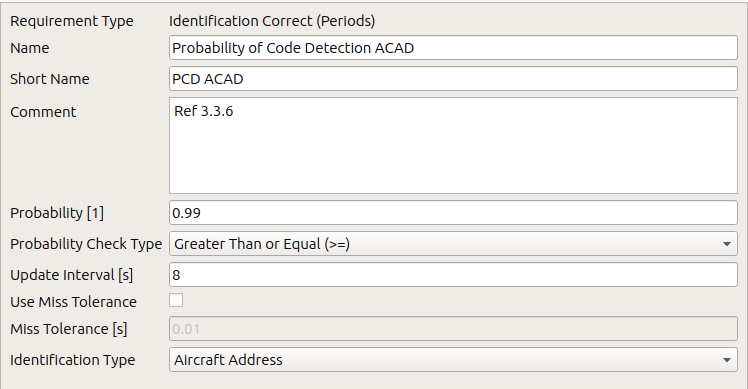
\includegraphics[width=14cm,frame]{figures/eval_req_id_correct_periods.png}
  \caption{Evaluation Identification Correct Periods requirement}
\end{figure}

\hl{TODO}

\subsubsection{Result Values}

\paragraph{Sector}

\begin{center}
 \begin{table}[H]
  \begin{tabularx}{\textwidth}{ | l | X |  l | }
    \hline
    \textbf{Name} & \textbf{Description} & \textbf{Example} \\ \hline
    Sector Layer & Name of the sector layer & fir\_body\_cut \\ \hline
    Reqirement Group & Name of the requirement group & En-Route \\ \hline
    Reqirement & Name of the requirement & Probability of Code Detection ACAD \\ \hline
    Num Results & Total number of results & 317 \\ \hline
    Num Usable Results & Number of usable results & 81 \\ \hline
    Num Unusable Results & Number of unusable results & 236 \\ \hline
    \#Updates/\#EUIs [1] & Total number update intervals & 4265 \\ \hline
    \#MUIs [1] & Number of missed update intervals & 134 \\ \hline
    PCAAD [\%] & Probability of Correct Aircraft Address Detection & 96.86 \\ \hline
    Condition &  & >= 99.00 \\ \hline
    Condition Fulfilled &  & Failed \\ \hline
    \#Single Targets &  & 81 \\ \hline
    \#Failed Single Targets &  & 2 \\ \hline
\end{tabularx}
\end{table}
\end{center}

\paragraph{Single Target}

\begin{center}
 \begin{table}[H]
  \begin{tabularx}{\textwidth}{ | l | X |  l | }
    \hline
    \textbf{Name} & \textbf{Description} & \textbf{Example} \\ \hline
    Use & To be used in results & true \\ \hline
    \#EUIs [1] & Expected Update Intervals & 35 \\ \hline
    \#MUIs [1] & Missed Update Intervals & 0 \\ \hline
    PCAAD [\%] & Probability of Correct Aircraft Address Detection & 100 \\ \hline
    Reference Period 1 & Time inside sector & [2023-06-30 16:03:14.056,2023-06-30 16:07:57.236] \\ \hline
    Condition &  & >= 99.00 \\ \hline
    Condition Fulfilled &  & Passed \\ \hline
\end{tabularx}
\end{table}
\end{center}

\subsection{Identification False}
\label{sec:eval_req_id_false} 

\subsubsection{Configuration}

\begin{figure}[H]
    \includegraphics[width=14cm,frame]{figures/eval_req_id_false.png}
  \caption{Evaluation Identification False requirement}
\end{figure}

The 'Identification False' requirement is used to calculate the probability of a target report having a false (secondary) identification. False in this context means there is identification data available, and it is not the same as in the reference. \\

\begin{itemize}  
\item Probability [1]: Probability of false identification
\item Probability Check Type: $\leq$
\item Require All False: If checked, all available secondary attributes be different than in the reference to count. If not checked, a single wrong secondary attribute is enough.
\item Use Mode 3/A Code: If the Mode 3/A code should be checked
\item Use Mode S Target Address: If the Mode S target address should be checked
\item Use Mode S Target Identification: If the Mode S target identification should be checked
\end{itemize}
\ \\

\subsubsection{Result Values}

\paragraph{Sector}

\begin{center}
 \begin{table}[H]
  \begin{tabularx}{\textwidth}{ | l | X |  l | }
    \hline
    \textbf{Name} & \textbf{Description} & \textbf{Example} \\ \hline
    Sector Layer & Name of the sector layer & fir\_cut\_sim \\ \hline
    Reqirement Group & Name of the requirement group & Mandatory \\ \hline
    Reqirement & Name of the requirement & Identification False \\ \hline
    Num Results & Total number of results & 728 \\ \hline
    Num Usable Results & Number of usable results & 107 \\ \hline
    Num Unusable Results & Number of unusable results & 621 \\ \hline
    Use & To be used in results & true \\ \hline
    \#Up [1] & Number of updates & 101685 \\ \hline
    \#NoRef [1] & Number of updates w/o reference position or identification & 7359 \\ \hline
    \#NoRefPos [1] & Number of updates w/o reference position  & 7359 \\ \hline
    \#NoRef [1] & Number of updates w/o reference identification & 0 \\ \hline
    \#PosInside [1] & Number of updates inside sector & 53997 \\ \hline
    \#PosOutside [1] & Number of updates outside sector & 40329 \\ \hline
    \#Unknown [1] & Number of updates unknown identification & 0 \\ \hline
    \#Correct [1] & Number of updates with correct identification & 53997 \\ \hline
    \#False [1] & Number of updates with false identification & 0 \\ \hline
    PF [\%] & Probability of identity false & 0 \\ \hline
    Condition &  & <= 1.00 \\ \hline
    Condition Fulfilled &  & Passed \\ \hline
\end{tabularx}
\end{table}
\end{center}

Also, a table is given for all single targets, sorted by PF.

\paragraph{Single Target}

\begin{center}
 \begin{table}[H]
  \begin{tabularx}{\textwidth}{ | l | X |  l | }
    \hline
    \textbf{Name} & \textbf{Description} & \textbf{Example} \\ \hline
    Use & To be used in results & true \\ \hline
    \#Up [1] & Number of updates & 566 \\ \hline
    \#NoRef [1] & Number of updates w/o reference position or identification & 51 \\ \hline
    \#NoRefPos [1] & Number of updates w/o reference position  & 51 \\ \hline
    \#NoRef [1] & Number of updates w/o reference identification & 0 \\ \hline
    \#PosInside [1] & Number of updates inside sector & 292 \\ \hline
    \#PosOutside [1] & Number of updates outside sector & 223 \\ \hline
    \#Unknown [1] & Number of updates unknown identification & 0 \\ \hline
    \#Correct [1] & Number of updates with correct identification & 292 \\ \hline
    \#False [1] & Number of updates with false identification & 0 \\ \hline
    PF [\%] & Probability of Mode 3/A false & 0 \\ \hline
    Condition &  & <= 1.00 \\ \hline
    Condition Fulfilled &  & Passed \\ \hline
\end{tabularx}
\end{table}
\end{center}

\subsection{Mode 3/A False}
\label{sec:eval_req_m3a_false} 

\subsubsection{Configuration}

\begin{figure}[H]
    \includegraphics[width=14cm,frame]{figures/eval_req_m3a_false.png}
  \caption{Evaluation Mode 3/A False requirement}
\end{figure}

The 'Mode 3/A False' requirement is used to calculate the probability of a target report having a false Mode 3/A code. False in this context means there is Mode 3/A information data available, and it is not the same as in the reference. Only values which are valid and not garbled are used. \\

\begin{itemize}  
\item Probability [1]: Probability of false Mode 3/A code
\item Probability Check Type: $\leq$
\end{itemize}
\ \\

\subsubsection{Result Values}

\paragraph{Sector}

\begin{center}
 \begin{table}[H]
  \begin{tabularx}{\textwidth}{ | l | X |  l | }
    \hline
    \textbf{Name} & \textbf{Description} & \textbf{Example} \\ \hline
    Sector Layer & Name of the sector layer & fir\_cut\_sim \\ \hline
    Reqirement Group & Name of the requirement group & Mandatory \\ \hline
    Reqirement & Name of the requirement & Mode A False \\ \hline
    Num Results & Total number of results & 728 \\ \hline
    Num Usable Results & Number of usable results & 106 \\ \hline
    Num Unusable Results & Number of unusable results & 622 \\ \hline
    Use & To be used in results & true \\ \hline
    \#Up [1] & Number of updates & 101669 \\ \hline
    \#NoRef [1] & Number of updates w/o reference position or code & 7353 \\ \hline
    \#NoRefPos [1] & Number of updates w/o reference position  & 7353 \\ \hline
    \#NoRef [1] & Number of updates w/o reference code & 0 \\ \hline
    \#PosInside [1] & Number of updates inside sector & 53987 \\ \hline
    \#PosOutside [1] & Number of updates outside sector & 40329 \\ \hline
    \#Unknown [1] & Number of updates unknown code & 198 \\ \hline
    \#Correct [1] & Number of updates with correct code & 53788 \\ \hline
    \#False [1] & Number of updates with false code & 1 \\ \hline
    PF [\%] & Probability of Mode 3/A false & 0 \\ \hline
    Condition &  & <= 1.00 \\ \hline
    Condition Fulfilled &  & Passed \\ \hline
\end{tabularx}
\end{table}
\end{center}

Also, a table is given for all single targets, sorted by PF.

\paragraph{Single Target}

\begin{center}
 \begin{table}[H]
  \begin{tabularx}{\textwidth}{ | l | X |  l | }
    \hline
    \textbf{Name} & \textbf{Description} & \textbf{Example} \\ \hline
    Use & To be used in results & true \\ \hline
    \#Up [1] & Number of updates & 732 \\ \hline
    \#NoRef [1] & Number of updates w/o reference position or code & 35 \\ \hline
    \#NoRefPos [1] & Number of updates w/o reference position  & 35 \\ \hline
    \#NoRef [1] & Number of updates w/o reference code & 0 \\ \hline
    \#PosInside [1] & Number of updates inside sector & 542 \\ \hline
    \#PosOutside [1] & Number of updates outside sector & 155 \\ \hline
    \#Unknown [1] & Number of updates unknown code & 5 \\ \hline
    \#Correct [1] & Number of updates with correct code & 536 \\ \hline
    \#False [1] & Number of updates with false code & 1 \\ \hline
    PF [\%] & Probability of Mode 3/A false & 0.19 \\ \hline
    Condition &  & <= 1.00 \\ \hline
    Condition Fulfilled &  & Passed \\ \hline
\end{tabularx}
\end{table}
\end{center}

\subsection{Mode 3/A Present}
\label{sec:eval_req_m3a_present} 

\subsubsection{Configuration}

\begin{figure}[H]
    \includegraphics[width=14cm,frame]{figures/eval_req_m3a_present.png}
  \caption{Evaluation Mode 3/A Present requirement}
\end{figure}

The 'Mode 3/A Present' requirement is used to calculate the probability of a target report having any Mode 3/A code. Present in this context means there is Mode 3/A information data available, irrespectively if correct or not. \\

\begin{itemize}  
\item Probability [1]: Probability of Mode 3/A code present
\item Probability Check Type: $\geq$
\end{itemize}
\ \\

\subsubsection{Result Values}

\paragraph{Sector}

\begin{center}
 \begin{table}[H]
  \begin{tabularx}{\textwidth}{ | l | X |  l | }
    \hline
    \textbf{Name} & \textbf{Description} & \textbf{Example} \\ \hline
    Sector Layer & Name of the sector layer & fir\_cut\_sim \\ \hline
    Reqirement Group & Name of the requirement group & Mandatory \\ \hline
    Reqirement & Name of the requirement & Mode A Present \\ \hline
    Num Results & Total number of results & 728 \\ \hline
    Num Usable Results & Number of usable results & 107 \\ \hline
    Num Unusable Results & Number of unusable results & 621 \\ \hline
    Use & To be used in results & true \\ \hline
    \#Up [1] & Number of updates & 101685 \\ \hline
    \#NoRef [1] & Number of updates w/o reference position & 7359 \\ \hline
    \#NoRefPos [1] & Number of updates w/o reference position  & 7359 \\ \hline
    \#PosInside [1] & Number of updates inside sector & 53997 \\ \hline
    \#PosOutside [1] & Number of updates outside sector & 40329 \\ \hline
    \#NoRefId [1] & Number of updates without reference code & 10 \\ \hline
    \#Present [1] & Number of updates with present tst code & 53789 \\ \hline
    \#Missing [1] & Number of updates with missing tst code & 198 \\ \hline
    PP [\%] & Probability of Mode 3/A present & 99.63 \\ \hline
    Condition &  & >= 98.00 \\ \hline
    Condition Fulfilled &  & Passed \\ \hline
\end{tabularx}
\end{table}
\end{center}

Also, a table is given for all single targets, sorted by PP.

\paragraph{Single Target}

\begin{center}
 \begin{table}[H]
  \begin{tabularx}{\textwidth}{ | l | X |  l | }
    \hline
    \textbf{Name} & \textbf{Description} & \textbf{Example} \\ \hline
    Use & To be used in results & true \\ \hline
    \#Up [1] & Number of updates & 956 \\ \hline
    \#NoRef [1] & Number of updates w/o reference position & 60 \\ \hline
    \#NoRefPos [1] & Number of updates w/o reference position  & 60 \\ \hline
    \#PosInside [1] & Number of updates inside sector & 467 \\ \hline
    \#PosOutside [1] & Number of updates outside sector & 429 \\ \hline
    \#NoRefId [1] & Number of updates without reference code & 0 \\ \hline
    \#Present [1] & Number of updates with present tst code & 456 \\ \hline
    \#Missing [1] & Number of updates with missing tst code & 11 \\ \hline
    PP [\%] & Probability of Mode 3/A present & 97.64 \\ \hline
    Condition &  & >= 98.00 \\ \hline
    Condition Fulfilled &  & Failed \\ \hline
\end{tabularx}
\end{table}
\end{center}

\subsection{Mode C Correct}
\label{sec:eval_req_mc_correct} 

\subsubsection{Configuration}

\begin{figure}[H]
    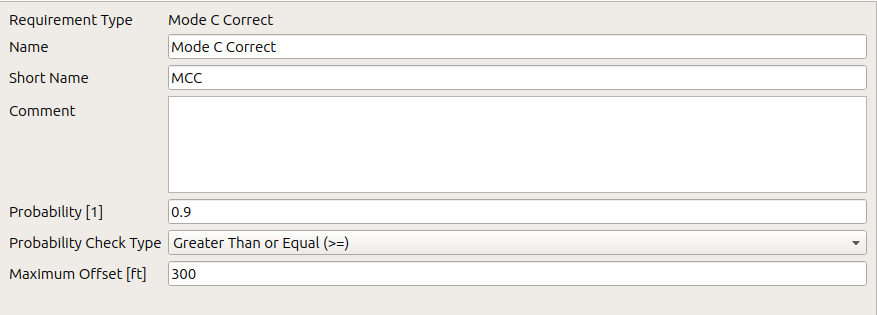
\includegraphics[width=14cm,frame]{figures/eval_req_mc_correct.png}
  \caption{Evaluation Mode C Correct requirement}
\end{figure}

The 'Mode C Correct' requirement is used to calculate the probability of a target report having a correct and valid Mode C code. Correct in this context means there is Mode C information data available, and it is the same as in the reference (within a certain threshold). Only values which are valid and not garbled are used. \\

\begin{itemize}  
\item Probability [1]: Probability of correct Mode C code
\item Probability Check Type: $\geq$
\item Maximum Offset [ft]: Maximum absolute distance between reference and test value to be counted as correct
\end{itemize}
\ \\

\subsubsection{Result Values}

\paragraph{Sector}

\begin{center}
 \begin{table}[H]
  \begin{tabularx}{\textwidth}{ | l | X |  l | }
    \hline
    \textbf{Name} & \textbf{Description} & \textbf{Example} \\ \hline
    Sector Layer & Name of the sector layer & fir\_body\_cut \\ \hline
    Reqirement Group & Name of the requirement group & Mandatory \\ \hline
    Reqirement & Name of the requirement & Mode C Correct \\ \hline
    Num Results & Total number of results & 317 \\ \hline
    Num Usable Results & Number of usable results & 84 \\ \hline
    Num Unusable Results & Number of unusable results & 233 \\ \hline
    \#Updates & Total number target reports & 86477 \\ \hline
    \#NoRef [1] & Number of updates w/o reference position or Mode C & 26095 \\ \hline
    \#NoRefPos [1] & Number of updates w/o reference position  & 26095 \\ \hline
    \#NoRef [1] & Number of updates w/o reference Mode C & 0 \\ \hline
    \#PosInside [1] & Number of updates inside sector & 33243 \\ \hline
    \#PosOutside [1] & Number of updates outside sector & 27139 \\ \hline
    \#CMC [1] & Number of updates with correct Mode C & 33207 \\ \hline
    \#NCMC [1] & Number of updates with no correct Mode C & 36 \\ \hline
    PC [\%] & Probability of correct Mode C & 99.89 \\ \hline
    Condition &  & >= 90.00 \\ \hline
    Condition Fulfilled &  & Passed \\ \hline
\end{tabularx}
\end{table}
\end{center}

Also, a table is given for all single targets, sorted by PC.

\paragraph{Single Target}

\begin{center}
 \begin{table}[H]
  \begin{tabularx}{\textwidth}{ | l | X |  l | }
    \hline
    \textbf{Name} & \textbf{Description} & \textbf{Example} \\ \hline
    Use & To be used in results & true \\ \hline
    \#Up [1] & Number of updates & 1110 \\ \hline
    \#NoRef [1] & Number of updates w/o reference position or Mode C & 1 \\ \hline
    \#NoRefPos [1] & Number of updates w/o reference position  & 1 \\ \hline
    \#NoRef [1] & Number of updates w/o reference Mode C & 0 \\ \hline
    \#PosInside [1] & Number of updates inside sector & 200 \\ \hline
    \#PosOutside [1] & Number of updates outside sector & 909 \\ \hline
    Max Dist. [ft] & Maximum offset & 300.00 \\ \hline
    \#CMC [1] & Number of updates with correct Mode C & 198 \\ \hline
    \#NCMC [1] & Number of updates with no correct Mode C & 2 \\ \hline
    PC [\%] & Probability of correct Mode C & 99 \\ \hline
    Condition &  & >= 90.00 \\ \hline
    Condition Fulfilled &  & Passed \\ \hline
\end{tabularx}
\end{table}
\end{center}

\subsection{Mode C Correct Periods}
\label{sec:eval_req_mc_correct_periods} 

\subsubsection{Configuration}

\begin{figure}[H]
    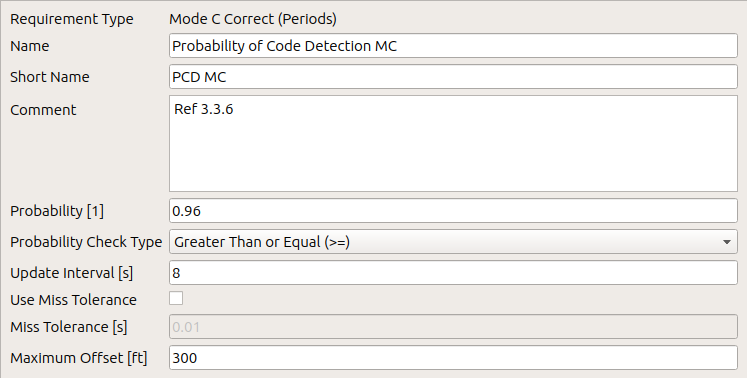
\includegraphics[width=14cm,frame]{figures/eval_req_mc_correct_periods.png}
  \caption{Evaluation Mode C Correct Periods requirement}
\end{figure}

\hl{TODO}

\subsubsection{Result Values}

\paragraph{Sector}

\begin{center}
 \begin{table}[H]
  \begin{tabularx}{\textwidth}{ | l | X |  l | }
    \hline
    \textbf{Name} & \textbf{Description} & \textbf{Example} \\ \hline
    Sector Layer & Name of the sector layer & fir\_body\_cut \\ \hline
    Reqirement Group & Name of the requirement group & En-Route \\ \hline
    Reqirement & Name of the requirement & Probability of Code Detection MC \\ \hline
    Num Results & Total number of results & 317 \\ \hline
    Num Usable Results & Number of usable results & 81 \\ \hline
    Num Unusable Results & Number of unusable results & 236 \\ \hline
    \#Updates/\#EUIs [1] & Total number update intervals & 4265 \\ \hline
    \#MUIs [1] & Number of missed update intervals & 0 \\ \hline
    PCMCD [\%] & Probability of Correct Mode C Detection & 100.00 \\ \hline
    Condition &  & >= 96.00 \\ \hline
    Condition Fulfilled &  & Passed \\ \hline
    \#Single Targets &  & 81 \\ \hline
    \#Failed Single Targets &  & 0 \\ \hline
\end{tabularx}
\end{table}
\end{center}

\paragraph{Single Target}

\begin{center}
 \begin{table}[H]
  \begin{tabularx}{\textwidth}{ | l | X |  l | }
    \hline
    \textbf{Name} & \textbf{Description} & \textbf{Example} \\ \hline
    Use & To be used in results & true \\ \hline
    \#EUIs [1] & Expected Update Intervals & 12 \\ \hline
    \#MUIs [1] & Missed Update Intervals & 0 \\ \hline
    PCMCD [\%] & Probability of Correct Mode C Detection & 100 \\ \hline
    Reference Period 1 & Time inside sector & [2023-06-30 16:06:17.256,2023-06-30 16:07:56.984] \\ \hline
    Condition &  & >= 96.00 \\ \hline
    Condition Fulfilled &  & Passed \\ \hline
\end{tabularx}
\end{table}
\end{center}

\subsection{Mode C False}
\label{sec:eval_req_mc_false} 

\subsubsection{Configuration}

\begin{figure}[H]
    \includegraphics[width=14cm,frame]{figures/eval_req_mc_false.png}
  \caption{Evaluation Mode C False requirement}
\end{figure}

The 'Mode C False' requirement is used to calculate the probability of a target report having a false Mode C code. False in this context means there is Mode C information data available, and the absolute difference between the test and the reference is larger than the given threshold. \\

\begin{itemize}  
\item Probability [1]: Probability of false Mode C code
\item Probability Check Type: $\leq$
\item Maximum Difference [ft]: Maximum altitude difference between the test and the reference, in feet
\end{itemize}
\ \\

\subsubsection{Result Values}

\paragraph{Sector}

\begin{center}
 \begin{table}[H]
  \begin{tabularx}{\textwidth}{ | l | X |  l | }
    \hline
    \textbf{Name} & \textbf{Description} & \textbf{Example} \\ \hline
    Sector Layer & Name of the sector layer & fir\_cut\_sim \\ \hline
    Reqirement Group & Name of the requirement group & Mandatory \\ \hline
    Reqirement & Name of the requirement & Mode C False \\ \hline
    Num Results & Total number of results & 728 \\ \hline
    Num Usable Results & Number of usable results & 107 \\ \hline
    Num Unusable Results & Number of unusable results & 621 \\ \hline
    Use & To be used in results & true \\ \hline
    \#Up [1] & Number of updates & 101685 \\ \hline
    \#NoRef [1] & Number of updates w/o reference position or code & 7363 \\ \hline
    \#NoRefPos [1] & Number of updates w/o reference position  & 7359 \\ \hline
    \#NoRef [1] & Number of updates w/o reference code & 4 \\ \hline
    \#PosInside [1] & Number of updates inside sector & 53997 \\ \hline
    \#PosOutside [1] & Number of updates outside sector & 40329 \\ \hline
    \#Unknown [1] & Number of updates unknown code & 40 \\ \hline
    \#Correct [1] & Number of updates with correct code & 53935 \\ \hline
    \#False [1] & Number of updates with false code & 18 \\ \hline
    PF [\%] & Probability of Mode C false & 0.03 \\ \hline
    Condition &  & <= 3.00 \\ \hline
    Condition Fulfilled &  & Passed \\ \hline
\end{tabularx}
\end{table}
\end{center}

Also, a table is given for all single targets, sorted by PF.

\paragraph{Single Target}

\begin{center}
 \begin{table}[H]
  \begin{tabularx}{\textwidth}{ | l | X |  l | }
    \hline
    \textbf{Name} & \textbf{Description} & \textbf{Example} \\ \hline
    Use & To be used in results & true \\ \hline
    \#Up [1] & Number of updates & 709 \\ \hline
    \#NoRef [1] & Number of updates w/o reference position or code & 30 \\ \hline
    \#NoRefPos [1] & Number of updates w/o reference position  & 30 \\ \hline
    \#NoRef [1] & Number of updates w/o reference code & 0 \\ \hline
    \#PosInside [1] & Number of updates inside sector & 591 \\ \hline
    \#PosOutside [1] & Number of updates outside sector & 88 \\ \hline
    \#Unknown [1] & Number of updates unknown code & 0 \\ \hline
    \#Correct [1] & Number of updates with correct code & 585 \\ \hline
    \#False [1] & Number of updates with false code & 6 \\ \hline
    PF [\%] & Probability of Mode C false & 1.02 \\ \hline
    Condition &  & <= 3.00 \\ \hline
    Condition Fulfilled &  & Passed \\ \hline
\end{tabularx}
\end{table}
\end{center}

\subsection{Mode C Present}
\label{sec:eval_req_mc_present} 

\subsubsection{Configuration}

\begin{figure}[H]
    \includegraphics[width=14cm,frame]{figures/eval_req_mc_present.png}
  \caption{Evaluation Mode C Present requirement}
\end{figure}

The 'Mode C Present' requirement is used to calculate the probability of a target report having any Mode C code. Present in this context means there is Mode C information data available, irrespectively if correct or not. \\

\begin{itemize}  
\item Probability [1]: Probability of Mode C code present
\item Probability Check Type: $\geq$
\end{itemize}
\ \\

\subsubsection{Result Values}

\paragraph{Sector}

\begin{center}
 \begin{table}[H]
  \begin{tabularx}{\textwidth}{ | l | X |  l | }
    \hline
    \textbf{Name} & \textbf{Description} & \textbf{Example} \\ \hline
    Sector Layer & Name of the sector layer & fir\_cut\_sim \\ \hline
    Reqirement Group & Name of the requirement group & Mandatory \\ \hline
    Reqirement & Name of the requirement & Mode C Present \\ \hline
    Num Results & Total number of results & 728 \\ \hline
    Num Usable Results & Number of usable results & 107 \\ \hline
    Num Unusable Results & Number of unusable results & 621 \\ \hline
    Use & To be used in results & true \\ \hline
    \#Up [1] & Number of updates & 101685 \\ \hline
    \#NoRef [1] & Number of updates w/o reference position & 7359 \\ \hline
    \#NoRefPos [1] & Number of updates w/o reference position  & 7359 \\ \hline
    \#PosInside [1] & Number of updates inside sector & 53997 \\ \hline
    \#PosOutside [1] & Number of updates outside sector & 40329 \\ \hline
    \#NoRefC [1] & Number of updates without reference code & 4 \\ \hline
    \#Present [1] & Number of updates with present tst code & 53953 \\ \hline
    \#Missing [1] & Number of updates with missing tst code & 40 \\ \hline
    PP [\%] & Probability of Mode C present & 99.93 \\ \hline
    Condition &  & >= 97.00 \\ \hline
    Condition Fulfilled &  & Passed \\ \hline
\end{tabularx}
\end{table}
\end{center}

Also, a table is given for all single targets, sorted by PP.

\paragraph{Single Target}

\begin{center}
 \begin{table}[H]
  \begin{tabularx}{\textwidth}{ | l | X |  l | }
    \hline
    \textbf{Name} & \textbf{Description} & \textbf{Example} \\ \hline
    Use & To be used in results & true \\ \hline
    \#Up [1] & Number of updates & 1041 \\ \hline
    \#NoRef [1] & Number of updates w/o reference position & 92 \\ \hline
    \#NoRefPos [1] & Number of updates w/o reference position  & 92 \\ \hline
    \#PosInside [1] & Number of updates inside sector & 406 \\ \hline
    \#PosOutside [1] & Number of updates outside sector & 543 \\ \hline
    \#NoRefC [1] & Number of updates without reference code & 0 \\ \hline
    \#Present [1] & Number of updates with present tst code & 398 \\ \hline
    \#Missing [1] & Number of updates with missing tst code & 8 \\ \hline
    PP [\%] & Probability of Mode C present & 98.03 \\ \hline
    Condition &  & >= 97.00 \\ \hline
    Condition Fulfilled &  & Passed \\ \hline
\end{tabularx}
\end{table}
\end{center}

\subsection{Position Across}
\label{sec:eval_req_pos_across} 

\subsubsection{Configuration}

\begin{figure}[H]
    \includegraphics[width=14cm,frame]{figures/eval_req_pos_across.png}
  \caption{Evaluation Position Across requirement}
\end{figure}

The 'Position Across' requirement is used to calculate the probability of a target report having an across-track error smaller than a defined threshold. The offset of the position (test vs. linear interpolated reference position) is used to calculate the error component across the track angle of the reference at the time. If the absolute value of this across-track position error is smaller or equal than the defined threshold, the target report is counted for the calculated probability PACOK. The PACOK must be greater or equal than the defined 'Probability' for the requirement to pass. \\

\begin{itemize}  
\item Probability [1]: Probability of acceptable across-track position
\item Probability Check Type: $\geq$
\item Maximum Absolute Value [m]: Maximum absolute across-track position difference between the test and the reference, in meters
\end{itemize}
\ \\

\subsubsection{Result Values}

\paragraph{Sector}

\begin{center}
 \begin{table}[H]
  \begin{tabularx}{\textwidth}{ | l | X |  l | }
    \hline
    \textbf{Name} & \textbf{Description} & \textbf{Example} \\ \hline
    Sector Layer & Name of the sector layer & fir\_cut\_sim \\ \hline
    Reqirement Group & Name of the requirement group & Mandatory \\ \hline
    Reqirement & Name of the requirement & Across \\ \hline
    Num Results & Total number of results & 728 \\ \hline
    Num Usable Results & Number of usable results & 107 \\ \hline
    Num Unusable Results & Number of unusable results & 621 \\ \hline
    Use & To be used in results & true \\ \hline
    \#Pos [1] & Number of updates & 101685 \\ \hline
    \#NoRef [1] & Number of updates w/o reference positions & 7359 \\ \hline
    \#PosInside [1] & Number of updates inside sector & 53997 \\ \hline
    \#PosOutside [1] & Number of updates outside sector & 40329 \\ \hline
    ACMin [m] & Minimum of across-track error & -444.23 \\ \hline
    ACMax [m] & Maximum of across-track error & 463.83 \\ \hline
    ACAvg [m] & Average of across-track error & 4.19 \\ \hline
    ACSDev [m] & Standard Deviation of across-track error & 24.81 \\ \hline
    ACVar [m$^2$] & Variance of across-track error & 615.60 \\ \hline
    \#ACOK [1] & Number of updates with across-track error & 52961 \\ \hline
    \#ACNOK [1] & Number of updates with unacceptable across-track error  & 1036 \\ \hline
    PACOK [\%] & Probability of acceptable across-track error & 98.08 \\ \hline
    Condition Across &  & >= 90.00 \\ \hline
    Condition Across Fulfilled &  & Passed \\ \hline
\end{tabularx}
\end{table}
\end{center}

Also, a table is given for all single targets, sorted by PACOK.

\paragraph{Single Target}

\begin{center}
 \begin{table}[H]
  \begin{tabularx}{\textwidth}{ | l | X |  l | }
    \hline
    \textbf{Name} & \textbf{Description} & \textbf{Example} \\ \hline
    Use & To be used in results & true \\ \hline
    \#Pos [1] & Number of updates & 515 \\ \hline
    \#NoRef [1] & Number of updates w/o reference positions & 45 \\ \hline
    \#PosInside [1] & Number of updates inside sector & 186 \\ \hline
    \#PosOutside [1] & Number of updates outside sector & 284 \\ \hline
    ACMin [m] & Minimum of across-track error & -28.77 \\ \hline
    ACMax [m] & Maximum of across-track error & 77.88 \\ \hline
    ACAvg [m] & Average of across-track error & 1.85 \\ \hline
    ACSDev [m] & Standard Deviation of across-track error & 12.83 \\ \hline
    ACVar [m$^2$] & Variance of across-track error & 164.55 \\ \hline
    \#ACOK [1] & Number of updates with across-track error & 185 \\ \hline
    \#ACNOK [1] & Number of updates with unacceptable across-track error  & 1 \\ \hline
    PACOK [\%] & Probability of acceptable across-track error & 99.46 \\ \hline
    Condition Across &  & >= 90.00 \\ \hline
    Condition Across Fulfilled &  & Passed \\ \hline
\end{tabularx}
\end{table}
\end{center}

\subsection{Position Along}
\label{sec:eval_req_pos_along} 

\subsubsection{Configuration}

\begin{figure}[H]
    \includegraphics[width=14cm,frame]{figures/eval_req_pos_along.png}
  \caption{Evaluation Position Along requirement}
\end{figure}

The 'Position Along' requirement is used to calculate the probability of a target report having an along-track error smaller than a defined threshold. The offset of the position (test vs. linear interpolated reference position) is used to calculate the error component along the track angle of the reference at the time. If the absolute value of this along-track position error is smaller or equal than the defined threshold, the target report is counted for the calculated probability PALOK. The PALOK must be greater or equal than the defined 'Probability' for the requirement to pass. \\

\begin{itemize}  
\item Probability [1]: Probability of acceptable along-track position
\item Probability Check Type: $\geq$
\item Maximum Absolute Value [m]: Maximum absolute along-track position difference between the test and the reference, in meters
\end{itemize}
\ \\

\subsubsection{Result Values}

\paragraph{Sector}

\begin{center}
 \begin{table}[H]
  \begin{tabularx}{\textwidth}{ | l | X |  l | }
    \hline
    \textbf{Name} & \textbf{Description} & \textbf{Example} \\ \hline
    Sector Layer & Name of the sector layer & fir\_cut\_sim \\ \hline
    Reqirement Group & Name of the requirement group & Mandatory \\ \hline
    Reqirement & Name of the requirement & Along \\ \hline
    Num Results & Total number of results & 728 \\ \hline
    Num Usable Results & Number of usable results & 107 \\ \hline
    Num Unusable Results & Number of unusable results & 621 \\ \hline
    Use & To be used in results & true \\ \hline
    \#Pos [1] & Number of updates & 101685 \\ \hline
    \#NoRef [1] & Number of updates w/o reference positions & 7359 \\ \hline
    \#PosInside [1] & Number of updates inside sector & 53997 \\ \hline
    \#PosOutside [1] & Number of updates outside sector & 40329 \\ \hline
    ALMin [m] & Minimum of along-track error & -1094.27 \\ \hline
    ALMax [m] & Maximum of along-track error & 828.16 \\ \hline
    ALAvg [m] & Average of along-track error & 18.37 \\ \hline
    ALSDev [m] & Standard Deviation of along-track error & 30.47 \\ \hline
    ALVar [m$^2$] & Variance of along-track error & 928.43 \\ \hline
    \#ALOK [1] & Number of updates with along-track error & 51854 \\ \hline
    \#ALNOK [1] & Number of updates with unacceptable along-track error  & 2143 \\ \hline
    PALOK [\%] & Probability of acceptable along-track error & 96.03 \\ \hline
    Condition Along &  & >= 90.00 \\ \hline
    Condition Along Fulfilled &  & Passed \\ \hline
\end{tabularx}
\end{table}
\end{center}

Also, a table is given for all single targets, sorted by PALOK.

\paragraph{Single Target}

\begin{center}
 \begin{table}[H]
  \begin{tabularx}{\textwidth}{ | l | X |  l | }
    \hline
    \textbf{Name} & \textbf{Description} & \textbf{Example} \\ \hline
    Use & To be used in results & true \\ \hline
    \#Pos [1] & Number of updates & 865 \\ \hline
    \#NoRef [1] & Number of updates w/o reference positions & 59 \\ \hline
    \#PosInside [1] & Number of updates inside sector & 482 \\ \hline
    \#PosOutside [1] & Number of updates outside sector & 324 \\ \hline
    ALMin [m] & Minimum of along-track error & -91.41 \\ \hline
    ALMax [m] & Maximum of along-track error & 100.38 \\ \hline
    ALAvg [m] & Average of along-track error & 42.52 \\ \hline
    ALSDev [m] & Standard Deviation of along-track error & 18.89 \\ \hline
    ALVar [m$^2$] & Variance of along-track error & 356.75 \\ \hline
    \#ALOK [1] & Number of updates with along-track error & 453 \\ \hline
    \#ALNOK [1] & Number of updates with unacceptable along-track error  & 29 \\ \hline
    PALOK [\%] & Probability of acceptable along-track error & 93.98 \\ \hline
    Condition Along &  & >= 90.00 \\ \hline
    Condition Along Fulfilled &  & Passed \\ \hline
\end{tabularx}
\end{table}
\end{center}

\subsection{Position Distance}
\label{sec:eval_req_pos_distance} 

\subsubsection{Configuration}

This requirement can be used in 2 variations:

\begin{figure}[H]
    \includegraphics[width=14cm,frame]{figures/eval_req_pos_distance_correct.png}
  \caption{Evaluation Position Distance requirement for correct positions}
\end{figure}

\begin{figure}[H]
    \includegraphics[width=14cm,frame]{figures/eval_req_pos_distance_false.png}
  \caption{Evaluation Position Distance requirement for false positions}
\end{figure}

The 'Position Distance' requirement is used to calculate the probability of a target report having a position error smaller or larger than a defined threshold. This two possibilities allow for calculation of a position correct or being false (e.g. outside an $5\sigma$ range of an expected error distribution). \\

The offset of the position (test vs. linear interpolated reference position) is used to calculate the Euklidian error distance. If the  value of this position error is fails the defined comparison threshold, the target report is counted for the calculated probability PCP (probability of check passed). The PCP must be in turn pass the check for the requirement to pass. \\

The 'Failed Values are of Interest' checkbox define if the target reports passing or failing the check are of interest.


\paragraph{Position Correct Variation}

\begin{itemize}  
\item Probability [1]: Probability of correct position
\item Probability Check Type: $\geq$
\item Threshold Value [m]: Maximum allowed distance from test target report to reference
\item Threshold Value Check Type: $\leq$, distance must be less or equal the given threshold
\item Failed Values are of Interest: Checked, the distances of interest are the ones not passing the check
\end{itemize}
\ \\

\paragraph{Position False Variation}

\begin{itemize}  
\item Probability [1]: Probability of false position
\item Probability Check Type: $\leq$
\item Threshold Value [m]: Minimum distance from test target report to reference
\item Threshold Value Check Type: $\geq$, distance must be greater or equal the given threshold
\item Failed Values are of Interest: Not checked, the distances of interest are the ones passing the check
\end{itemize}
\ \\

\subsubsection{Result Values}

\paragraph{Sector}

\begin{center}
 \begin{table}[H]
  \begin{tabularx}{\textwidth}{ | l | X |  l | }
    \hline
    \textbf{Name} & \textbf{Description} & \textbf{Example} \\ \hline
    Sector Layer & Name of the sector layer & fir\_cut\_sim \\ \hline
    Reqirement Group & Name of the requirement group & Mandatory \\ \hline
    Reqirement & Name of the requirement & Position Correct \\ \hline
    Num Results & Total number of results & 728 \\ \hline
    Num Usable Results & Number of usable results & 107 \\ \hline
    Num Unusable Results & Number of unusable results & 621 \\ \hline
    Use & To be used in results & true \\ \hline
    \#Pos [1] & Number of updates & 101685 \\ \hline
    \#NoRef [1] & Number of updates w/o reference positions & 7359 \\ \hline
    \#PosInside [1] & Number of updates inside sector & 53997 \\ \hline
    \#PosOutside [1] & Number of updates outside sector & 40329 \\ \hline
    DMin [m] & Minimum of distance & 0.09 \\ \hline
    DMax [m] & Maximum of distance & 1115.68 \\ \hline
    DAvg [m] & Average of distance & 34.06 \\ \hline
    DSDev [m] & Standard Deviation of distance & 27.19 \\ \hline
    DVar [m$^2$] & Variance of distance & 739.18 \\ \hline
    \#CF [1] & Number of updates with failed comparison & 291 \\ \hline
    \#CP [1] & Number of updates with passed comparison  & 53706 \\ \hline
    PCP [\%] & Probability of passed comparison & 99.46 \\ \hline
    Condition &  & >= 90.00 \\ \hline
    Condition Fulfilled &  & Passed \\ \hline
\end{tabularx}
\end{table}
\end{center}

Also, a table is given for all single targets, sorted by PCP.

\paragraph{Single Target}

\begin{center}
 \begin{table}[H]
  \begin{tabularx}{\textwidth}{ | l | X |  l | }
    \hline
    \textbf{Name} & \textbf{Description} & \textbf{Example} \\ \hline
    Use & To be used in results & true \\ \hline
    \#Pos [1] & Number of updates & 927 \\ \hline
    \#NoRef [1] & Number of updates w/o reference positions & 52 \\ \hline
    \#PosInside [1] & Number of updates inside sector & 646 \\ \hline
    \#PosOutside [1] & Number of updates outside sector & 229 \\ \hline
    DMin [m] & Minimum of distance & 4.14 \\ \hline
    DMax [m] & Maximum of distance & 284.87 \\ \hline
    DAvg [m] & Average of distance & 81.87 \\ \hline
    DSDev [m] & Standard Deviation of distance & 34.43 \\ \hline
    DVar [m$^2$] & Variance of distance & 1185.18 \\ \hline
    \#CF [1] & Number of updates with failed comparison & 25 \\ \hline
    \#CP [1] & Number of updates with  passed comparison & 621 \\ \hline
    PCP [\%] & Probability of passed comparison & 96.13 \\ \hline
    Condition &  & >= 90.00 \\ \hline
    Condition Fulfilled &  & Passed \\ \hline
\end{tabularx}
\end{table}
\end{center}

\subsection{Position Distance RMS}
\label{sec:eval_req_pos_distance_rms} 

\subsubsection{Configuration}

\begin{figure}[H]
    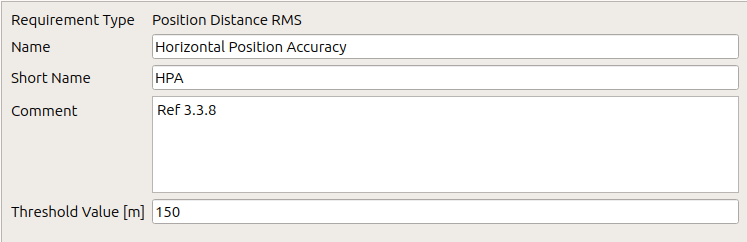
\includegraphics[width=14cm,frame]{figures/eval_req_pos_distance_rms.png}
  \caption{Evaluation Position Latency requirement}
\end{figure}

The 'Position Distance' requirement is used to calculate if the RMS position error is larger than a defined threshold. \\

The offset of the position (test vs. linear interpolated reference position) is used to calculate the RMS error distance for a number of target reports. The requirement is failed if the the calculated RMS value is larger than the defined threshold. \\

\begin{itemize}  
\item Threshold Value [m]: Maximum allowed RMS
\end{itemize}

\subsubsection{Result Values}

\paragraph{Sector}

\begin{center}
 \begin{table}[H]
  \begin{tabularx}{\textwidth}{ | l | X |  l | }
    \hline
    \textbf{Name} & \textbf{Description} & \textbf{Example} \\ \hline
    Sector Layer & Name of the sector layer & fir\_cut\_sim \\ \hline
    Reqirement Group & Name of the requirement group & Mandatory \\ \hline
    Reqirement & Name of the requirement & Position Correct \\ \hline
    Num Results & Total number of results & 728 \\ \hline
    Num Usable Results & Number of usable results & 107 \\ \hline
    Num Unusable Results & Number of unusable results & 621 \\ \hline
    Use & To be used in results & true \\ \hline
    \#Pos [1] & Number of updates & 101685 \\ \hline
    \#NoRef [1] & Number of updates w/o reference positions & 7359 \\ \hline
    \#PosInside [1] & Number of updates inside sector & 53997 \\ \hline
    \#PosOutside [1] & Number of updates outside sector & 40329 \\ \hline
    DMin [m] & Minimum of distance & 0.23 \\ \hline
    DMax [m] & Maximum of distance & 515.87 \\ \hline
    DAvg [m] & Average of distance & 29.25 \\ \hline
    DSDev [m] & Standard Deviation of distance & 23.12 \\ \hline
    DVar [$m^2$] & Variance of distance & 534.32 \\ \hline
    RMS & Root mean square & 37.28 \\ \hline
    \#CF [1] & Number of updates with failed comparison & 9 \\ \hline
    \#CP [1] & Number of updates with passed comparison  & 33234 \\ \hline
    Condition &  & <= 350.000000 \\ \hline
    Condition Fulfilled &  & Passed \\ \hline
\end{tabularx}
\end{table}
\end{center}

Also, a table is given for all single targets, sorted by RMS.

\paragraph{Single Target}

\begin{center}
 \begin{table}[H]
  \begin{tabularx}{\textwidth}{ | l | X |  l | }
    \hline
    \textbf{Name} & \textbf{Description} & \textbf{Example} \\ \hline
    Use & To be used in results & true \\ \hline
    \#Pos [1] & Number of updates & 927 \\ \hline
    \#NoRef [1] & Number of updates w/o reference positions & 52 \\ \hline
    \#PosInside [1] & Number of updates inside sector & 646 \\ \hline
    \#PosOutside [1] & Number of updates outside sector & 229 \\ \hline
    DMin [m] & Minimum of distance & 58.89 \\ \hline
    DMax [m] & Maximum of distance & 371.66 \\ \hline
    DAvg [m] & Average of distance & 110.69 \\ \hline
    DSDev [m] & Standard Deviation of distance & 59.38 \\ \hline
    DVar [$m^2$] & Variance of distance & 125.61 \\ \hline
    RMS & Root mean square & 3525.42 \\ \hline
    \#CF [1] & Number of updates with failed comparison & 1 \\ \hline
    \#CP [1] & Number of updates with passed comparison & 31 \\ \hline
    Condition &  & <= 350.000000 \\ \hline
    Condition Fulfilled &  & Passed \\ \hline
\end{tabularx}
\end{table}
\end{center}

\subsection{Position Latency}
\label{sec:eval_req_pos_latency} 

\subsubsection{Configuration}

\begin{figure}[H]
    \includegraphics[width=14cm,frame]{figures/eval_req_pos_latency.png}
  \caption{Evaluation Position Latency requirement}
\end{figure}

The 'Position Latency' requirement is used to calculate the probability of a target report having a time-latency error smaller than a defined threshold. The offset of the position (test vs. linear interpolated reference position) is used to calculate the error component along the track angle of the reference at the time, which divided by the negative speed gives the latency. If the absolute value of this latency is smaller or equal than the defined threshold, the target report is counted for the calculated probability PLTOK. The PLTOK must be greater or equal than the defined 'Probability' for the requirement to pass. \\

\begin{itemize}  
\item Probability [1]: Probability of acceptable position latency
\item Probability Check Type: $\geq$
\item Maximum Absolute Value [s]: Maximum absolute latency, in seconds
\end{itemize}
\ \\

\subsubsection{Result Values}

\paragraph{Sector}

\begin{center}
 \begin{table}[H]
  \begin{tabularx}{\textwidth}{ | l | X |  l | }
    \hline
    \textbf{Name} & \textbf{Description} & \textbf{Example} \\ \hline
    Sector Layer & Name of the sector layer & fir\_cut\_sim \\ \hline
    Reqirement Group & Name of the requirement group & Mandatory \\ \hline
    Reqirement & Name of the requirement & Latency \\ \hline
    Num Results & Total number of results & 728 \\ \hline
    Num Usable Results & Number of usable results & 107 \\ \hline
    Num Unusable Results & Number of unusable results & 621 \\ \hline
    Use & To be used in results & true \\ \hline
    \#Pos [1] & Number of updates & 101685 \\ \hline
    \#NoRef [1] & Number of updates w/o reference positions & 7359 \\ \hline
    \#PosInside [1] & Number of updates inside sector & 53997 \\ \hline
    \#PosOutside [1] & Number of updates outside sector & 40329 \\ \hline
    LTMin [s] & Minimum of latency & -00:00:02.758 \\ \hline
    LTMax [s] & Maximum of latency & 00:00:04.790 \\ \hline
    LTAvg [s] & Average of latency & -00:00:00.081 \\ \hline
    LTSDev [s] & Standard Deviation of latency & 00:00:00.146 \\ \hline
    LTVar [s$^2$] & Variance of latency & 00:00:00.021 \\ \hline
    \#LTOK [1] & Number of updates with latency & 44216 \\ \hline
    \#LTNOK [1] & Number of updates with unacceptable latency  & 9781 \\ \hline
    PLTOK [\%] & Probability of acceptable latency & 81.89 \\ \hline
    Condition Latency &  & >= 90.00 \\ \hline
    Condition Latency Fulfilled &  & Failed \\ \hline
\end{tabularx}
\end{table}
\end{center}

Also, a table is given for all single targets, sorted by PLTOK.

\paragraph{Single Target}

\begin{center}
 \begin{table}[H]
  \begin{tabularx}{\textwidth}{ | l | X |  l | }
    \hline
    \textbf{Name} & \textbf{Description} & \textbf{Example} \\ \hline
    Use & To be used in results & true \\ \hline
    \#Pos [1] & Number of updates & 1729 \\ \hline
    \#NoRef [1] & Number of updates w/o reference positions & 142 \\ \hline
    \#PosInside [1] & Number of updates inside sector & 1469 \\ \hline
    \#PosOutside [1] & Number of updates outside sector & 118 \\ \hline
    LTMin [s] & Minimum of latency & -00:00:00.590 \\ \hline
    LTMax [s] & Maximum of latency & 00:00:00.431 \\ \hline
    LTAvg [s] & Average of latency & -00:00:00.092 \\ \hline
    LTSDev [s] & Standard Deviation of latency & 00:00:00.085 \\ \hline
    LTVar [s$^2$] & Variance of latency & 00:00:00.007 \\ \hline
    \#LTOK [1] & Number of updates with latency & 1324 \\ \hline
    \#LTNOK [1] & Number of updates with unacceptable latency  & 145 \\ \hline
    PLTOK [\%] & Probability of acceptable latency & 90.13 \\ \hline
    Condition Latency &  & >= 90.00 \\ \hline
    Condition Latency Fulfilled &  & Passed \\ \hline
\end{tabularx}
\end{table}
\end{center}

\subsection{Speed}
\label{sec:eval_req_speed} 

\subsubsection{Configuration}

\begin{figure}[H]
    \includegraphics[width=14cm,frame]{figures/eval_req_speed.png}
  \caption{Evaluation Speed requirement}
\end{figure}

The 'Speed' requirement is used to calculate the probability of a target report having an speed error smaller than a defined threshold. The difference of the speed (test speed vs. speed based on reference positions) is calculated, and if its absolute value is smaller or equal than the defined threshold, the target report is counted for the calculated probability PCP (probability of check passed). The PCP must be greater or equal than the defined 'Probability' for the requirement to pass. \\

In another variation, if the 'Use Percent Threshold if Higher' checkbox is set, the check is changed for faster speeds. If the 'Threshold Percent' value times the calculated speed is larger or equal the dewfined threshold value, then threshold value is changed to value of the 'Threshold Percent' value times the calculated speed. This means that for higher speeds, an accuracy with the given percentage is required. \\

\begin{itemize}  
\item Probability [1]: Probability of false Mode C code
\item Probability Check Type: $\geq$
\item Speed Offset Value [m/s]: Maximum absolute speed difference between the test and the reference, in meters per second
\item Use Percent Threshold if Higher: Defines if the percent-based accuracy should be used for higher speeds
\item Threshold Percent [\%]: Percent threshold
\item Threshold Value Check Type: $\leq$, speed difference must be less or equal the given threshold
\item Failed Values are of Interest: Checked, the speed values of interest are the ones not passing the check
\end{itemize}
\ \\

\subsubsection{Result Values}

\paragraph{Sector}

\begin{center}
 \begin{table}[H]
  \begin{tabularx}{\textwidth}{ | l | X |  l | }
    \hline
    \textbf{Name} & \textbf{Description} & \textbf{Example} \\ \hline
    Sector Layer & Name of the sector layer & fir\_cut\_sim \\ \hline
    Reqirement Group & Name of the requirement group & Mandatory \\ \hline
    Reqirement & Name of the requirement & Speed \\ \hline
    Num Results & Total number of results & 728 \\ \hline
    Num Usable Results & Number of usable results & 107 \\ \hline
    Num Unusable Results & Number of unusable results & 621 \\ \hline
    Use & To be used in results & true \\ \hline
    \#Pos [1] & Number of updates & 101685 \\ \hline
    \#NoRef [1] & Number of updates w/o reference speeds & 7359 \\ \hline
    \#PosInside [1] & Number of updates inside sector & 53997 \\ \hline
    \#PosOutside [1] & Number of updates outside sector & 40329 \\ \hline
    \#NoTstData [1] & Number of updates without tst speed data & 0 \\ \hline
    OMin [m/s] & Minimum of speed offset & 0.00 \\ \hline
    OMax [m/s] & Maximum of speed offset & 1114.58 \\ \hline
    OAvg [m/s] & Average of speed offset & 3.59 \\ \hline
    OSDev [m/s] & Standard Deviation of speed offset & 7.62 \\ \hline
    OVar [m$^2$/s$^2$] & Variance of speed offset & 58.01 \\ \hline
    \#CF [1] & Number of updates with failed comparison & 38 \\ \hline
    \#CP [1] & Number of updates with passed comparison  & 53959 \\ \hline
    PCP [\%] & Probability of passed comparison & 99.93 \\ \hline
    Condition &  & >= 90.00 \\ \hline
    Condition Fulfilled &  & Passed \\ \hline
\end{tabularx}
\end{table}
\end{center}

Also, a table is given for all single targets, sorted by PCP.

\paragraph{Single Target}

\begin{center}
 \begin{table}[H]
  \begin{tabularx}{\textwidth}{ | l | X |  l | }
    \hline
    \textbf{Name} & \textbf{Description} & \textbf{Example} \\ \hline
    Use & To be used in results & true \\ \hline
    \#Pos [1] & Number of updates & 1795 \\ \hline
    \#NoRef [1] & Number of updates w/o reference speeds & 131 \\ \hline
    \#PosInside [1] & Number of updates inside sector & 949 \\ \hline
    \#PosOutside [1] & Number of updates outside sector & 715 \\ \hline
    \#NoTstData [1] & Number of updates without tst speed data & 0 \\ \hline
    OMin [m/s] & Minimum of speed offset & 0.00 \\ \hline
    OMax [m/s] & Maximum of speed offset & 56.07 \\ \hline
    OAvg [m/s] & Average of speed offset & 5.23 \\ \hline
    OSDev [m/s] & Standard Deviation of speed offset & 5.60 \\ \hline
    OVar [m$^2$/s$^2$] & Variance of speed offset & 31.34 \\ \hline
    \#CF [1] & Number of updates with failed comparison & 2 \\ \hline
    \#CP [1] & Number of updates with  passed comparison & 947 \\ \hline
    PCP [\%] & Probability of passed comparison & 99.79 \\ \hline
    Condition &  & >= 90.00 \\ \hline
    Condition Fulfilled &  & Passed \\ \hline
\end{tabularx}
\end{table}
\end{center}
